\documentclass[12pt,oneside]{fithesis}
%\documentclass[12pt,draft,oneside]{fithesis}
\usepackage[utf8]{inputenc}
\usepackage[IL2]{fontenc}
\usepackage[plainpages=false, pdfpagelabels]{hyperref}
\usepackage{paralist}
\usepackage{graphicx}
%\usepackage{url}
\thesistitle{Design and implementation of a social network for making acquaintances}
\thesissubtitle{Bachelor thesis}
\thesisstudent{Marek Bryša}
\thesiswoman{false}
\thesisfaculty{fi}
\thesislang{en}
\thesisyear{spring 2012}
\thesisadvisor{doc. Ing. Michal Brandejs, CSc.}

\begin{document}
\FrontMatter
\ThesisTitlePage

\begin{ThesisDeclaration}
\DeclarationText
\AdvisorName
\end{ThesisDeclaration}

\begin{ThesisThanks}
Thanks
\end{ThesisThanks}

abstract

\MainMatter
\tableofcontents
\chapter*{Introduction}
\chapter{Design}
\section{Existing social networks for making acquaintances}
	\subsection{PlentyofFish}
		PlentyofFish (\url{http://www.plentyoffish.com/}) was founded in 2003 in Canada. It generates most of it's revenue through advertising and some premium services. Unfortunately, it currently only serves users from Canada, UK, US, Australia, Ireland, New Zealand, Spain, France, Italy and Germany so the author could not sign up at all.
		
		From the publicly available information, it allows users to create a profile, search for others, message and chat with others. A 'Chemisty test' and some other methods of finding a match are offered, but without exlaining precisely how they work.\cite{website:pof}
		\subsection{Match.com}
		Match.com (\url{http://www.match.com}) was launched in 1995 and is one of the oldest networks. It requires a paid subscription of ranging from 34.90EUR for one month  to 77.40EUR for 6 months.
		
		After signing up, the user is asked to upload a profile photo and fill in a detailed questionnaire about his or her character, interests, activities and relationships and preferences. Based on this information, the system tries to find the best matching partner. The user can then add the match to his or her favourites, follow their profile and message them. There is a special option to 'wink' at them, which can be used to quickly bring attention of the match and wait for their response to quickly assess their general interest without the need to send a message.\cite{website:match}
		
		\subsection{OkCupid}
		OkCupid (\url{http://www.okcupid.com}) started in 2004. It claims to be the fastest growing site. TODO: use dating???\\
		It is ad-supported and the essential features are free to use. A paid subscription called 'A-list' is also available for 14.95USD/month. It removes the ads, allows for advaced search, changing of username etc.
		
		Matches can be found through search using general criteria or by filling out questionnaires. A user can also create a his own questions, set their importance and expected answers. When another user fills them in, the system calculates a match percentage. This process is probably unique to OkCupid.\cite{website:okcupid}
		\subsection{eHarmony}
		eHarmony (\url{http://www.eharmony.com}) is a paid service that was launched in 2000. It claims to have more than 33 million members. Subscriptions cost from 59.95USD for a month  to 239.4USD for 12 months. It is primarily focused on finding a partner for marriage.
		
		The service uses personality tests, mathematical matching and expert advice to find the best match. There are separate subsites targeted for specific social groups such as Asians, Christians, Jews, gays and  lesbians etc. A new user has to fill in a very detailed questionnaire about his current status, personality and preferences.\cite{website:eharmony}
\section{User data protection}
	When using this kind of social networks, the user usually has to provide information about himself that is very sensitive and even intimate. Protection of this data is therefore a very serious concern.
	
	The data is very valuable beyond it's original intent to find the best match. It can be used for instance to precisely target advertisments, give offers to buy new products and so on. Hence it is essential that the user is made clear how the information he enters on a website is used or if it is disclosed to third parties.
	
	The user should also have the ability to choose what data is shared with other users. In the best case this control should be very fine, i.e. the user should not be forced to share information in blocks, should be able to deny concrete user from viewing his profile or parts of his profile etc. There should also be a simple tool to preview one's profile in the way others can see it.
	
	If a user deletes any data on his profile, it should be physically deleted from all the servers as well, unless it is expressly stated otherwise (e.g. for backup purposes).
	
	Any changes to the privacy policy of a website should be only done with sufficent prior notice and preferabely be opt-in. The user must have the ability to close his account. In this context, it also very important for the user to able to simply download all his data in a package.
	
	The language of the privacy policy should be as simple as possible, for every user to clearly understand it. Almost noone will read a lengthy legal text, which can lead to unfortunate misunderstandings later.
	
	It goes almost without saying that the servers must be well protected from hacker attacks, especially when they contain this kind of sensitive data. A successful attack would not only harm the users, but probably mark the end for the website. Ideally there should be a regular security audit that the users can review.

\section{The idea}
	TODO:
	\cite{Finkel01012012}
	From the research of existing social networks for making acquaintances we can conclude the following points and issues:
	\begin{itemize}
		\item The target audience are single people from their late 20's to about 60 years old.
		\item Many require a paid subscription to access even the most basic functionality.
		\item All require new users to fill in a long, detailed and intimate questionnaire. This can discourage many users.
		\item Therefore all collect very sensitive user data that could be potentially misused.
		\item All offer a method to quickly find a matching partner, but then require an action from one of the users to make a first contact. Some users might have trouble finding courage to do so.
	\end{itemize}

	To solve most of these issues, the author has come up with this idea for the new social network:
	\begin{itemize}
		\item The users will provide only general information: e-mail address, gender, year of birth, approximate location (county level), interest in men or women and a single profile photo.
		\item Based on simple search criteria such as age range, relative location to them (i.e. same county, neighbouring counties, etc.), they will browse profile pictures of other users one by one and mark the ones they like.
		\item Only once two users match their mark, both will be notified, added to their contact lists and be able to engage in real-time chat. Then they can get to know each other and possibly arrange a meeting.
	\end{itemize}
	
	This way only very little information is gathered in the database, which brings the user data privacy problems to minimum and it is not needed to fill in any lengthy questionnaires. User need not be shy when marking people they like, because until the mark is matched, the other person will not know about it.
	
	However this also brings some new issues. Because the marking of others is essentially only based on their looks, the target audience is going to be reduced to users for whom it is an important criteria. That means mostly younger people seeking fun rather than a serious relationship.
\chapter{Implementation}

\section{Technologies}
%http://www.okcupid.com/about/technology
	It is very important to choose the right technology for the implementation of a project. We need to find the most suitable web application framework and a data store, if one is not hard-wired into the framework. The author has devised the following criteria for the evaluation of available technologies:
	\begin{itemize}
		\item \textbf{Availability for commercial use free of charge}\\
			Because of budgetary constrains, the technology must be free for commercial use. The project may later generate revenue through the use advertising.
		\item \textbf{General suitability for the project}\\
			It must facilitate creation of a website. It is expected that there will be a lot of HTTP requests that will make only little chages to the database, e.g. marking of photos a user likes. The data model will be quite simple. There must be an easy way of making HTTP push\footnote{"HTTP server push (also known as HTTP streaming) is a mechanism for sending data from a web server to a web browser." \url{http://en.wikipedia.org/wiki/HTTP_push}, {2012-08-04}} communication to enable real-time chat. 
		\item \textbf{Runtime speed, resource intensity and stability}\\
			Again due to the low bugdet, the software must utilize the hardware as efficiently as possible. The framework should have a good track record of runtime stability and error recovery.
		\item \textbf{Scalability}\\
			The user base could potentially grow very rapidly. It is therefore essential that all the system can match the growth cost efficiently.
		\item \textbf{Ease of development and developer community size}\\
			It should be easy to implement the project and good documentation is welcome. The framework should have a good community with which a developer can try to solve issues.
		\item \textbf{Code stability}\\
			The technologies should be past their rapid development phases and the core APIs should be stable. This minimizes the effort needed to transition the project to a newer version of the framework. 
		\item \textbf{Innovation factor}\\
			Younger technologies are preffered as their use can lead to innovation and discovery of new approaches to problems.
	\end{itemize}
	Because of the first criterion, our interest shall only be in open source frameworks.
	\subsection{General suitability for the project}
		The author is skilled in JavaScript, PHP, Python and Ruby, so we will further examine frameworks based on those languages. All have been used for HTTP server programming for a long time, except for JavaScript, which has emerged in recent years in the Node.js platform.\\
		\begin{table}[htb]
		\begin{tabular}{|r||p{2.2cm}|p{2.2cm}|p{2.1cm}|p{2.2cm}|}
			\hline 
			\rule[-1ex]{0pt}{2.5ex} & Node.js & PHP & Python & Ruby \\ 
			\hline\hline
			\rule[-1ex]{0pt}{2.5ex} Simple & Express.js & plain PHP & CherryPy & Sinatra \\ 
			\hline 
			\rule[-1ex]{0pt}{2.5ex} Full MVC & Locomotive, Railway.js & Zend, CakePHP & Dajngo, web2py & Ruby on Rails \\ 
			\hline 
		\end{tabular}
		\caption{Classification of web frameworks}
		\label{table:wf}
		\end{table}
	
		Table \ref{table:wf} shows a basic classification of selected web frameworks by programming language and complexity of features they provide. Simple frameworks generally only provide a way to route HTTP requests to methods, parse HTTP headers and to send a response. Other features can be added on using plugins or modules. Full MVC\footnote{Model-View-Controller} frameworks also have an ORM\footnote{Object-Relational Mapping} engine for models and generate HTML views using a templating engine.
		
		Because the project's uncomplicated data model would not utilize the complex feature set of full MVC frameworks and those could limit flexibility, we will further only focus on the simple ones, i.e. Express.js, plain PHP, CherryPy and Sinatra.
		
	\subsection{Runtime speed, resource intensity and stability}
		Let us first compare speed of the languages and their virtual machines themselves. We can use results from \emph{The Computer Language Benchmarks Game} \cite{website:bench}. It uses several algorithms written in different programming languages to measure their speed.
		
		\begin{figure}[htb]
	  \centering
	    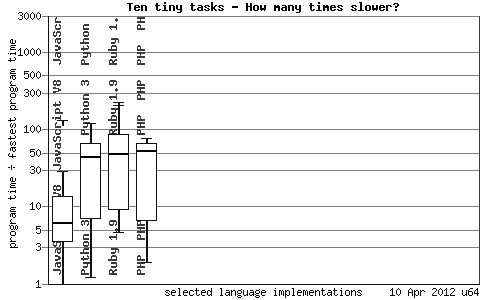
\includegraphics[width=0.7\textwidth]{bench2.png}
		  \caption{Language benchmark of V8 Engine, Python 3, Ruby 1.9 and PHP 5.4.0}
		  \label{fig:bench1}
		\end{figure}
		
		A box plot of the benchmark is shown in figure \ref{fig:bench1}. The vertical axis means how many times the language is slower than the fastest one (Intel Fortran 12.1). Out of the languages under consideration, Node.js on average 6 times faster than the rest\footnote{Node.js uses the V8 Engine internally}. 
		
		In this section we will benchmark the platforms still left in the comparison to determine their speed. All the tests will be run on a dual-core i686 Linux 3.2.11 PC with 4GB of RAM.
	
	
	\subsection{Data store}		
		The decision to use simple web framework gives us a free hand in choosing a separate data store. The traditional choice is an SQL database, e.g. MySQL and PostgreSQL. Lately NoSQL databases (MongoDB, CouchDB etc.) and  advanced key-value storages such as Redis have come into focus. In a recent paper \emph{Social-data storage-systems} \cite{Ruflin2011} that compares all of above, no clear winner is given.
		
		The author has chosen Redis. "Redis is an open source, advanced key-value store. It is often referred to as a data structure server since keys can contain strings, hashes, lists, sets and sorted sets."\cite{website:redis} Redis keep the entire database in memory with optional regular persistent storage snapshots, which allows for very fast read/write access and good reliability.	Benchmarks such as \cite{website:ruturaj} show that Redis is about eight times af fast as MySQL when it comes to simple operations.
		
		One of the drawbacks is that Redis mostly has simple commands so complex operations are difficult to program.
		
		The innovation factor is high because Redis is usually not used as a single storage for all the data. As a bonus, Redis contains a simple publisher-subscriber functionality, which will come handy when implementing the real-time chat.
\section{Basic functionality}
	\subsection{User registration}
	\subsection{Profile photo upload}
	\subsection{Acquaintance selection}
	\subsection{Notifications}
	\subsection{Chat}
\section{Implementation in detail}
	\subsection{Security}
	\subsection{I18n}
	\subsection{Geolocation}
	\subsection{Graphical design}
\chapter{Conclusion}

% Následují další kapitoly a podkapitoly, popřípadě závěr, dodatky, 
% seznam literatury či použitých obrázků nebo tabulek.

\bibliographystyle{plain}  % bibliografický styl 
\bibliography{bp} % soubor s citovanými
                           % položkami bibliografie 

\end{document}